\documentclass[11pt]{article}

\usepackage[margin=1in]{geometry}
\usepackage{amsmath,amssymb,amsfonts}
\usepackage{booktabs}
\usepackage{bm}
\usepackage{graphicx}
\usepackage{xcolor}
\usepackage[colorlinks=true,linkcolor=blue!50!black,citecolor=blue!50!black,urlcolor=blue!50!black]{hyperref}
\usepackage{listings}
\usepackage{caption}
\usepackage{subcaption}
\usepackage{tcolorbox}

\graphicspath{{out/}}

\lstset{
  basicstyle=\ttfamily\small,
  breaklines=true,
  columns=fullflexible,
  showstringspaces=false,
  frame=single,
  framesep=4pt,
  framerule=0.3pt,
  rulecolor=\color{black!30},
  numbers=none,
}

\newtcolorbox{example}[1][]{
  colback=blue!3, colframe=blue!40!black, boxrule=0.4pt,
  arc=2pt, left=6pt, right=6pt, top=4pt, bottom=4pt,
  title={Worked example}, fonttitle=\bfseries, #1
}

\newcommand{\Score}{A_{\text{score}}}
\newcommand{\Adisj}{A_{\text{disj}}}
\newcommand{\Aact}{A_{\text{act}}}
\newcommand{\Acons}{A_{\text{cons}}}
\newcommand{\Anec}{A_{\text{nec}}}
\newcommand{\IoU}{\operatorname{IoU}}

\title{A Score for Robot Helpers When Tasks Have Multiple\\Acceptable Time Windows}
\author{Metric side quest --- AURA evaluation}
\date{\today}

\begin{document}
\maketitle

\begin{abstract}
We are building a robot assistant that decides \emph{when} to step in
and help a person with a task. To check whether the robot does the
right thing at the right time, we compare its decisions against a
recording of when a human teleoperator chose to step in --- the
``ground truth''. Our old comparison method assumes there is exactly
one correct moment for each helping action. In reality, many helping
actions could be done in any of several time windows. This note
describes a new ground-truth format and a new score that allows for
those multiple correct windows, and shows that the new score behaves
sensibly on a small worked example and on our existing hand-layup
recording.
\end{abstract}

\section{Why we need a new score}
\label{sec:motivation}

Imagine you are watching a robot help a person make tea. The person is
the main worker; the robot only steps in for a few specific subtasks
(say, ``hand over the kettle'', ``open the cupboard''). To check
whether the robot's timing is good, we wrote down a list of the
moments when an expert teleoperator chose to step in, and we score the
robot by comparing its actions to this list.

Up to now, each entry in that list looked like this:
\begin{quote}
``\textbf{hand over the kettle} should happen between \textbf{10\,s and
15\,s}.''
\end{quote}
Just one window per subtask. This works, but it lies in two ways:

\paragraph{Lie 1: there is often more than one correct window.}
``Hand over the kettle'' could be done before the person fills the
teapot, \emph{or} during a brief pause while they wait for the water
to boil. Both are reasonable. If the robot picks the second window and
our list only mentions the first, we wrongly mark it as wrong.

\paragraph{Lie 2: a subtask might need to happen in two parts.}
``Bring the resin and then put it back'' is one logical subtask, but
the robot has to be in two different places at two different times.
A single window cannot describe that.

We need a richer description of ``when is it OK to do this''.
Section~\ref{sec:gt} introduces such a description, and
Section~\ref{sec:metric} introduces a score that uses it.

\section{The new ground-truth format}
\label{sec:gt}

We give each subtask a small tree of acceptable schedules:

\begin{itemize}
  \item A \textbf{phase} is a single time window, e.g.\ ``between
    10\,s and 15\,s''. It is the smallest unit.
  \item An \textbf{option} is a list of phases that all have to
    happen for that option to count. ``Bring the resin (between 5\,s
    and 10\,s) \emph{and} put it back (between 25\,s and 30\,s)'' is
    one option made of two phases.
  \item An \textbf{intervention} (one subtask) is a list of options.
    Only \emph{one} option needs to happen, but every phase inside
    that one option has to happen. ``Either bring the resin and put
    it back \emph{or} bring the hardener and put it back'' is one
    intervention with two options.
\end{itemize}

\noindent
You can read it as: \emph{an intervention is a choice of option, and
an option is a list of windows that all have to be filled.} If we
write it out symbolically, it looks like this:
\begin{equation}
  \underbrace{\bigvee_{k=1}^{M_i}}_{\text{pick \textbf{one} option}} \;
  \underbrace{\bigwedge_{j=1}^{L_{i,k}}}_{\text{satisfy \textbf{every} phase in it}} \;
  \underbrace{t_{i,k,j} \in [s_{i,k,j}, e_{i,k,j}]}_{\text{within this window}}.
  \label{eq:dtn-constraint}
\end{equation}
Here $i$ indexes the subtask, $k$ the option, $j$ the phase. The
``$\bigvee$'' means \emph{or}; the ``$\bigwedge$'' means \emph{and}.
Don't worry too much about the symbols --- the important point is
``one option, but all its phases''.

\subsection{Same idea, in JSON}

The format on disk just mirrors the structure above.
Listing~\ref{lst:toy} is the small example we will use throughout
this note. Three subtasks, two options each, and some options have
two phases.

\begin{lstlisting}[caption={Our toy ground truth: three subtasks, two options each. Notice how some windows are reused across different options on purpose.},label=lst:toy]
"interventions": [
  {"id": "task_1",
   "options": [
     {"phases": [{"t_start": 5,  "t_end": 10},
                 {"t_start": 25, "t_end": 30}]},
     {"phases": [{"t_start": 10, "t_end": 15},
                 {"t_start": 35, "t_end": 40}]}
   ]},
  {"id": "task_2",
   "options": [
     {"phases": [{"t_start": 0,  "t_end": 5},
                 {"t_start": 10, "t_end": 15}]},
     {"phases": [{"t_start": 10, "t_end": 15},
                 {"t_start": 25, "t_end": 30}]}
   ]},
  {"id": "task_3",
   "options": [
     {"phases": [{"t_start": 0,  "t_end": 5}]},
     {"phases": [{"t_start": 35, "t_end": 40}]}
   ]}
]
\end{lstlisting}

\subsection{Why the example is interesting}

The robot can only do one thing at a time. When we lay all the windows
on a single timeline, we see that some choices clash:

\begin{example}
Suppose the robot picks ``option~A'' for every subtask. Then:
\begin{itemize}
  \item task~1 wants $[5,10]$ and $[25,30]$.
  \item task~2 wants $[0,5]$ and $[10,15]$.
  \item task~3 wants $[0,5]$.
\end{itemize}
But task~2 and task~3 both want $[0,5]$ --- the robot can't be in two
places at once! So picking ``option~A everywhere'' is impossible. The
\emph{only} fully-feasible plan is ``A, A, B'' (task~1 option~A, task~2
option~A, task~3 option~B), which uses windows
$\{[5,10], [25,30]\}$, $\{[0,5], [10,15]\}$, and $\{[35,40]\}$ ---
none of these clash.
\end{example}

This is the key behaviour we want our score to capture: \emph{the
robot has to pick options that fit together}, not just options that
individually look fine.

\subsection{The old format still works}

Our hand-layup recording was written in the old format (one window per
subtask). The new format is a strict extension --- we can read an old
file and pretend each subtask has ``one option containing one phase''.
On such a file, the new score behaves like the old one. Nothing breaks.

\section{The new score}
\label{sec:metric}

We compare the robot's predictions against the ground truth on four
separate dimensions, then combine them. Each dimension is a number
between 0 (terrible) and 1 (perfect).
\begin{equation}
  \Score
  = w_{\text{disj}}\Adisj
  + w_{\text{act}}\Aact
  + w_{\text{cons}}\Acons
  + w_{\text{nec}}\Anec.
  \label{eq:composite}
\end{equation}
We default to weights $0.4, 0.2, 0.2, 0.2$ --- coverage matters
slightly more than the rest, and the four weights add up to 1 so the
final score also lies between 0 and 1. The four pieces are explained
below; informally,
\begin{description}
  \item[$\Adisj$ (\emph{coverage})] --- did the robot fill the
    required time windows?
  \item[$\Aact$ (\emph{action})] --- did it do the right \emph{kind}
    of action in those windows?
  \item[$\Acons$ (\emph{consistency})] --- do its choices fit
    together, or do they clash with the one-thing-at-a-time
    constraint?
  \item[$\Anec$ (\emph{necessity})] --- did it act \emph{only} when
    asked, or also a lot of useless extra times?
\end{description}

\subsection{Background on overlap (IoU)}

Most of the dimensions need a way to ask ``how much do these two time
windows overlap?''. The standard answer is the
\emph{intersection-over-union} (IoU):
\begin{equation*}
  \IoU\!\bigl([a,b], [c,d]\bigr) =
  \frac{\text{length of overlap}}{\text{length of the union}}.
\end{equation*}
IoU is 1 when the two windows are exactly the same and 0 when they
do not overlap at all.

\begin{example}
$\IoU([5,10], [5,10]) = 1$ (identical).
$\IoU([5,10], [7,12]) = 3/7 \approx 0.43$ (they share $[7,10]$, length
3, and together they cover $[5,12]$, length 7).
$\IoU([5,10], [20,25]) = 0$ (no overlap at all).
\end{example}

\subsection{$\Adisj$: did the robot fill the right windows?}
\label{sec:adisj}

For each subtask we look only at predictions whose action label
matches that subtask. Then for \emph{each option} of that subtask we
ask: how well does the robot's best matching prediction fill each
phase of this option, on average?

The option with the highest score wins, and that score is the
subtask's contribution to $\Adisj$. The overall $\Adisj$ is just the
average across all subtasks.

\begin{example}
Suppose for task~1, the robot predicted a ``task~1''-labelled action
in $[5,10]$ and another in $[25,30]$. Then:
\begin{itemize}
  \item Option~A has phases $[5,10]$ and $[25,30]$. Best IoU per phase
    is 1.0 and 1.0. Mean = 1.0.
  \item Option~B has phases $[10,15]$ and $[35,40]$. Best IoU per
    phase is 0 and 0. Mean = 0.
\end{itemize}
Best option is A with score 1.0. So task~1 contributes 1.0 to
$\Adisj$, and we say the robot ``selected option~A'' for task~1.
\end{example}

So $\Adisj$ rewards proposals that land inside one of the allowed
schedules, and ignores how the robot describes its plan in words --- we
infer which option it meant from \emph{when} it acted.

\subsection{$\Aact$: did it do the right kind of action?}
\label{sec:aact}

For each prediction, we find the GT phase that overlaps it the most
(highest IoU). If the robot's action label matches the action label of
that phase, the prediction is ``correct''. $\Aact$ is the fraction of
overlapping predictions that are correct.

\textbf{Tie-breaking matters.} Sometimes two phases from
\emph{different} subtasks share the same window (e.g.\ task~1
option~B's first phase and task~2 option~A's second phase are both
$[10,15]$). If the robot's prediction at $[10,15]$ is labelled
``task~2'', we should not penalise it just because task~1 also
\emph{could} use that window. So when several phases tie at the
highest IoU, we count the prediction as correct if any of them shares
its action label.

\subsection{$\Acons$: do the chosen options fit together?}
\label{sec:acons}

Recall that the robot can only do one thing at a time. After we have
inferred which option each subtask used (from $\Adisj$), we check
whether any pair of those chosen options collides --- i.e.\ has
phases overlapping in time.

We use the worst pairwise IoU among phases from \emph{different}
subtasks as the penalty:
\begin{equation*}
  \Acons = 1 - \bigl(\text{worst pairwise IoU between selected phases of different subtasks}\bigr).
\end{equation*}
If no two selected phases overlap, $\Acons = 1$. If two of them
overlap exactly, $\Acons = 0$.

\begin{example}
The toy GT has exactly one fully-feasible combination: A, A, B (task~1
option~A, task~2 option~A, task~3 option~B). On that combination, no
pair of selected phases overlaps and $\Acons = 1$. On the combination
A, A, A (which is what the ``always pick option 0'' adversary
chooses), task~2 phase $[0,5]$ and task~3 phase $[0,5]$ are identical,
so the worst pair has IoU 1 and $\Acons = 0$.
\end{example}

This is the dimension that the old score could not see at all.

\subsection{$\Anec$: did it intervene only when asked?}
\label{sec:anec}

Take \emph{all} the phase windows in the GT (across every option of
every subtask) and union them into one big set of allowed time
$\Phi$. Then ask: out of the total time the robot spent acting, how
much of it was inside $\Phi$?
\begin{equation*}
  \Anec = \frac{\text{total prediction time spent inside }\Phi}{\text{total prediction time}}.
\end{equation*}
A robot that fires all over the place gets low $\Anec$. A robot that
acts only inside legitimate windows gets $\Anec = 1$. By convention,
$\Anec = 1$ when the robot makes no predictions at all (you cannot
make a false alarm if you say nothing --- a silent robot is punished
by $\Adisj$ instead).

\section{The adversaries}
\label{sec:adversaries}

To check whether the score actually distinguishes good behaviour from
bad behaviour, we wrote thirteen \emph{adversaries} --- fake robots
each designed to fail in one specific way. The full list is in
Table~\ref{tab:adversaries}.

\begin{table}[ht]
\centering
\small
\begin{tabular}{lp{0.66\linewidth}}
\toprule
\textbf{Adversary} & \textbf{What it does} \\
\midrule
Oracle (consistent)   & Picks an option for each subtask such that no two chosen phases clash. Fires exactly those phases. \emph{Should score perfectly}. \\
Oracle (first option) & Always picks option index 0. Same correct \emph{timing}, but its choices may clash. \\
Conflict-prone        & On purpose picks options whose phases overlap as much as possible. \\
Phase-collapsed       & Like the consistent oracle, but only fires the \emph{first} phase of each option. \\
Half-coverage         & Like the consistent oracle, but covers only every other subtask. \\
Wrong-skill           & Right windows, but every prediction's label is shifted to the \emph{next} subtask's label. \\
Near-miss timing      & Consistent oracle shifted by $+1.5$\,s. \\
Far-shifted           & Consistent oracle shifted by $+8$\,s. \\
Premature firer       & Consistent oracle shifted by $-1.5$\,s. \\
Over-extender         & Right starts; every phase end is padded by $+4$\,s. \\
One-shot blanket      & A single prediction covering the whole task duration. \\
Spammer               & Rapid-fire short predictions of the most-common action label. \\
Silent                & Empty prediction track --- never acts. \\
\bottomrule
\end{tabular}
\caption{The thirteen adversaries used to validate the new score.}
\label{tab:adversaries}
\end{table}

\section{Results}
\label{sec:results}

\subsection{Toy three-task example}

Figure~\ref{fig:toy} stacks the GT (top three rows) above each
adversary's predictions. Table~\ref{tab:toy} gives the four-dimension
breakdown.

\begin{figure}[ht]
  \centering
  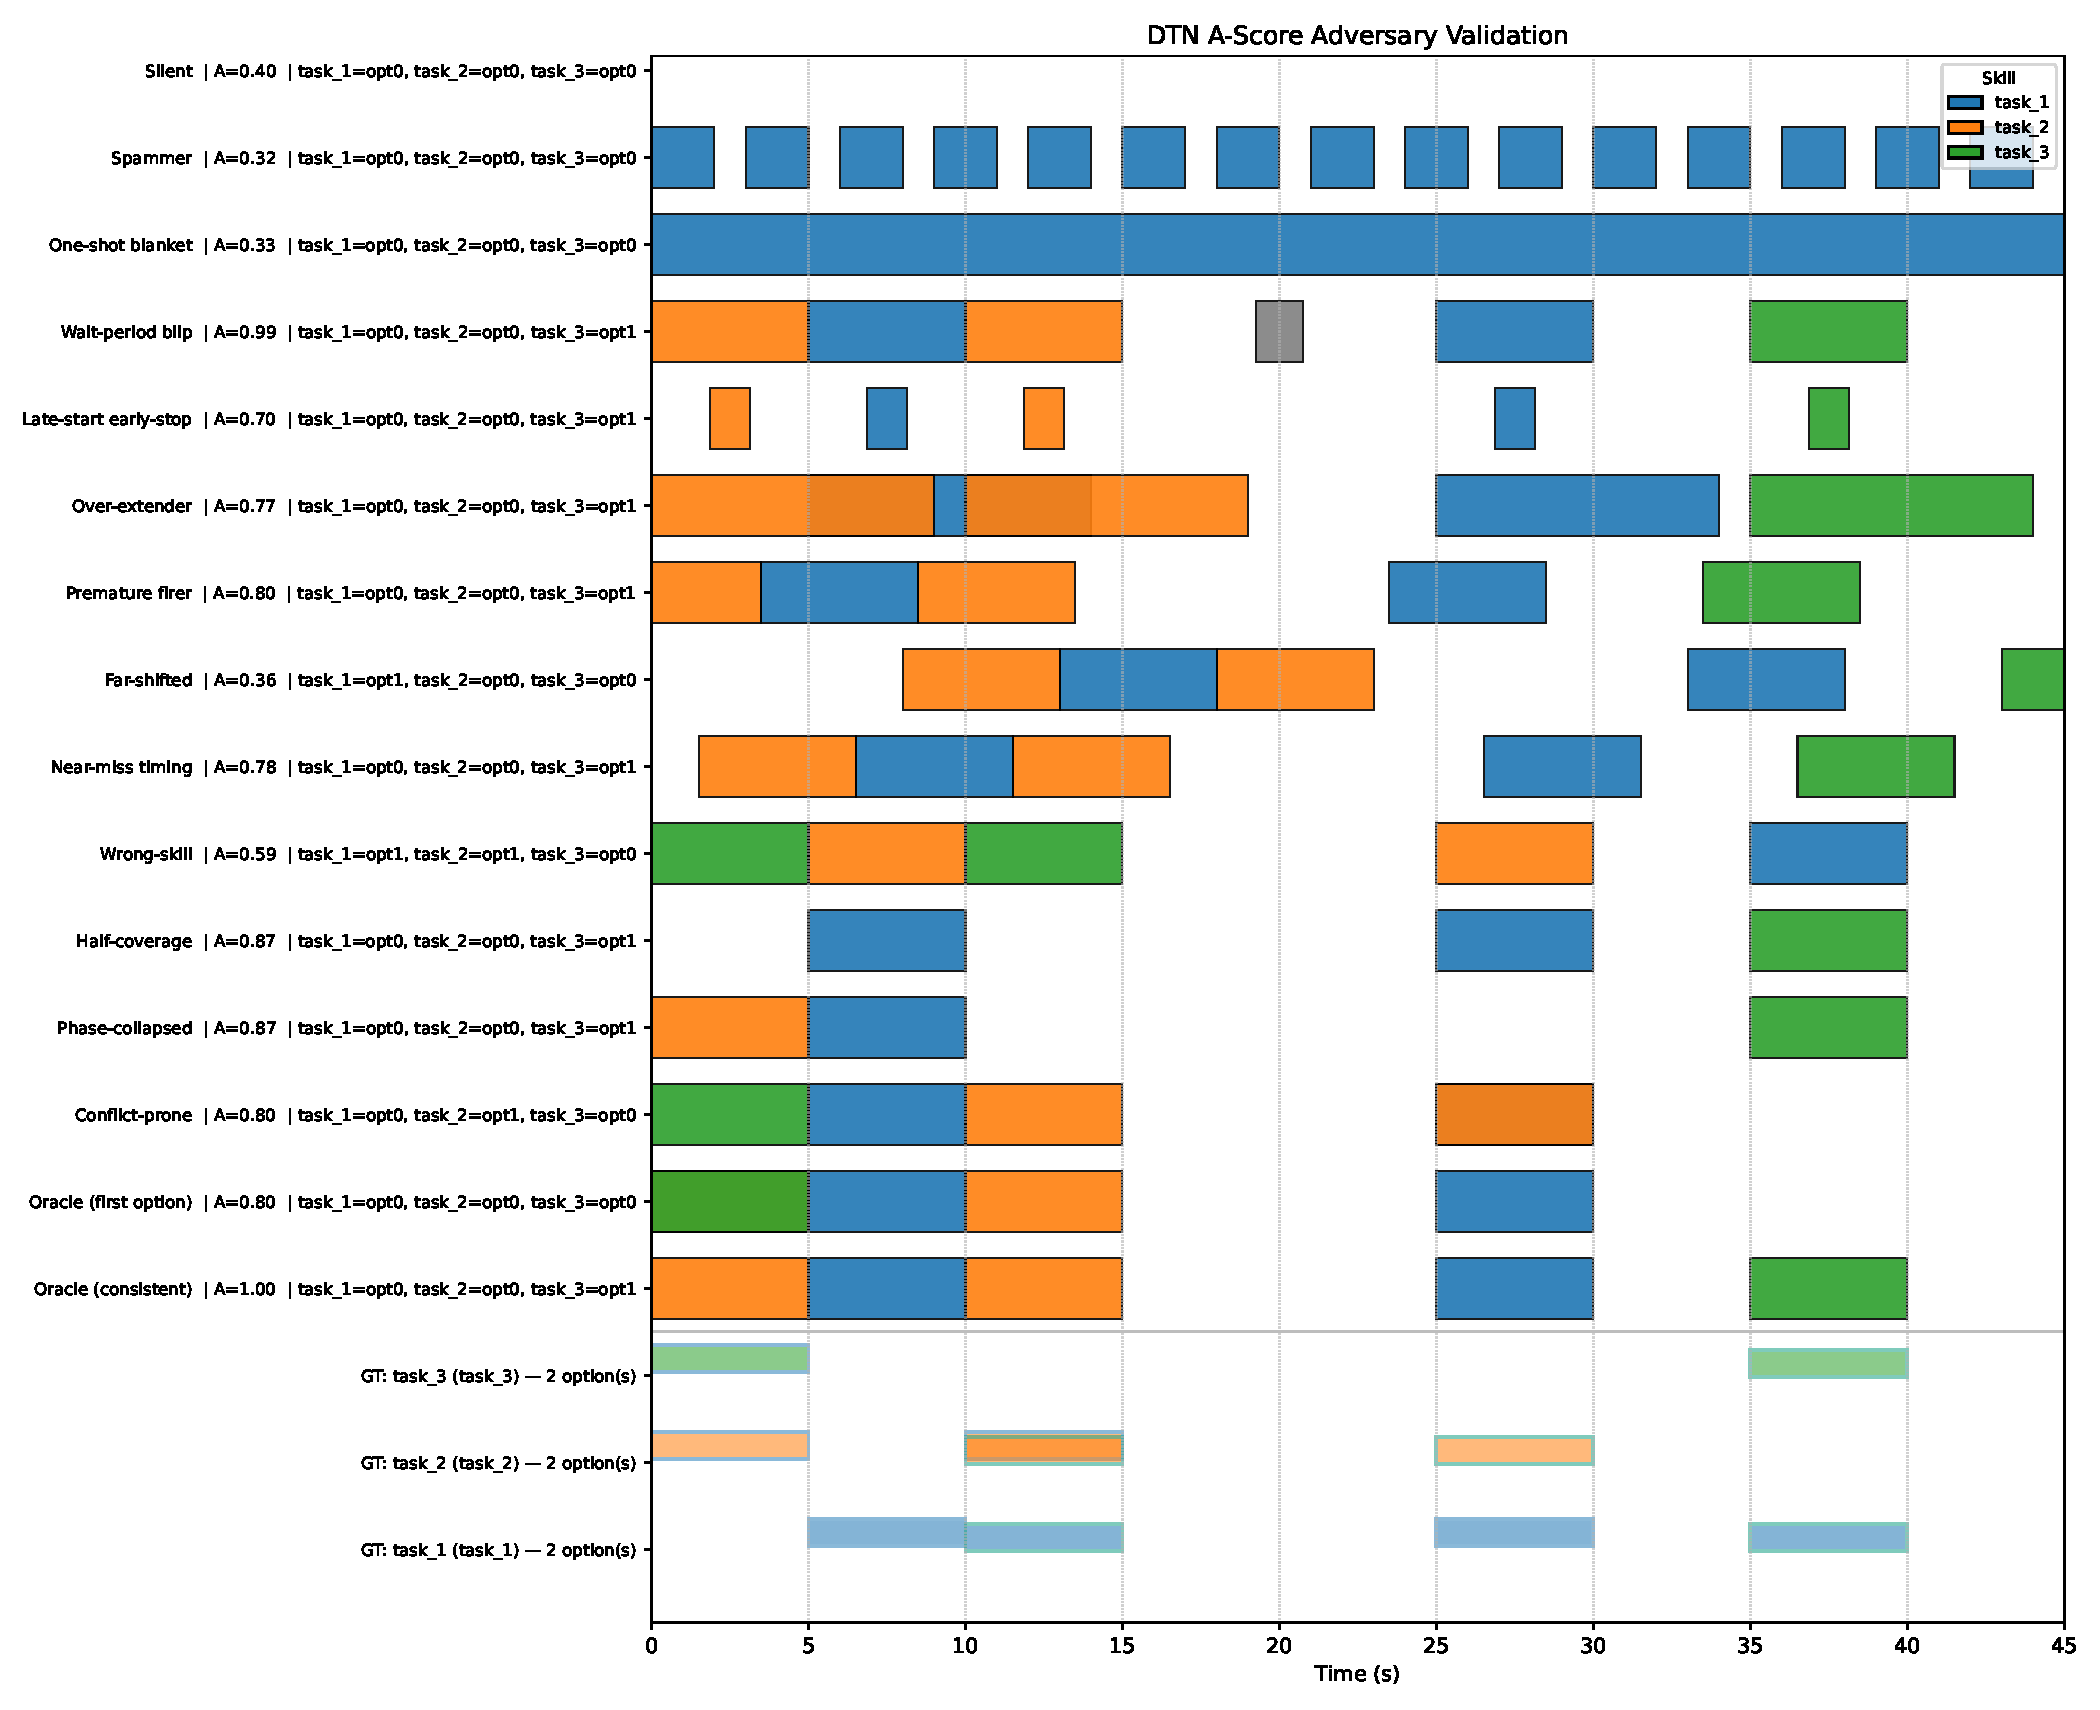
\includegraphics[width=\linewidth]{fig_dtn_adversaries.pdf}
  \caption{Toy DTN. Top three rows: the ground truth, with each
  subtask's two options drawn one above the other (different edge
  colours = different options). Lower rows: each adversary's
  predictions. The label on each row reports the final score and the
  option the metric \emph{inferred} that the adversary was aiming at.}
  \label{fig:toy}
\end{figure}

\begin{table}[ht]
\centering
\small
\begin{tabular}{lrrrrr}
\toprule
\textbf{Adversary} & $\bm{\Adisj}$ & $\bm{\Aact}$ & $\bm{\Acons}$ & $\bm{\Anec}$ & $\bm{\Score}$ \\
\midrule
Oracle (consistent)   & 1.00 & 1.00 & 1.00 & 1.00 & \textbf{1.00} \\
Oracle (first option) & 1.00 & 1.00 & 0.00 & 1.00 & 0.80 \\
Conflict-prone        & 1.00 & 1.00 & 0.00 & 1.00 & 0.80 \\
Phase-collapsed       & 0.67 & 1.00 & 1.00 & 1.00 & 0.87 \\
Half-coverage         & 0.67 & 1.00 & 1.00 & 1.00 & 0.87 \\
Wrong-skill           & 0.67 & 0.60 & 0.00 & 1.00 & 0.59 \\
Near-miss timing      & 0.54 & 1.00 & 1.00 & 0.82 & 0.78 \\
Far-shifted           & 0.19 & 1.00 & 0.00 & 0.45 & 0.37 \\
Premature firer       & 0.57 & 1.00 & 1.00 & 0.87 & 0.80 \\
Over-extender         & 0.56 & 1.00 & 1.00 & 0.73 & 0.77 \\
One-shot blanket      & 0.04 & 1.00 & 0.00 & 0.56 & 0.33 \\
Spammer               & 0.13 & 0.78 & 0.00 & 0.53 & 0.32 \\
Silent                & 0.00 & 1.00 & 0.00 & 1.00 & 0.40 \\
\bottomrule
\end{tabular}
\caption{Score breakdown on the toy DTN
(weights $w = (0.40, 0.20, 0.20, 0.20)$).}
\label{tab:toy}
\end{table}

\paragraph{What the table tells us.}
The four dimensions each surface a different kind of failure:
\begin{itemize}
  \item \textbf{Coverage vs.\ consistency.} ``Oracle (first option)''
    and ``Conflict-prone'' fill every required window with the right
    action label, so $\Adisj = 1$ and $\Aact = 1$. But the options
    they pick overlap each other, so $\Acons$ drops to 0. They end up
    below the consistent oracle. \emph{This is the failure mode the
    old score could not see.}
  \item \textbf{Coverage vs.\ correctness.} ``Wrong-skill'' has the
    right windows but the wrong labels, which both lowers $\Aact$
    \emph{and} confuses the option-selection logic, dragging $\Acons$
    down too.
  \item \textbf{Coverage vs.\ necessity.} ``Spammer'' and ``one-shot
    blanket'' flood the timeline; their $\Anec$ correctly drops below
    0.6 because most of their predicted time lies outside any
    legitimate window.
  \item \textbf{Silent strategy.} The silent adversary scores
    $\Score = 0.4$ --- not zero, because by convention the
    ``correctness'' and ``necessity'' axes give credit for not making
    bad predictions. But $\Adisj = 0$ keeps it well below any
    adversary that actually does something useful.
\end{itemize}

\subsection{Hand-layup recording (old-format ground truth)}

Our existing hand-layup ground truth has only one option per subtask
and one phase per option (the old format). On this kind of input,
$\Acons$ is automatically 1 (you cannot create a clash if there is
only one possible choice), and $\Adisj$ becomes plain mean phase IoU
--- exactly the same as the old timing axis. Figure~\ref{fig:layup}
and Table~\ref{tab:layup} confirm this: the relative ranking of
adversaries on the hand-layup recording matches what we would expect
from the old score.

\begin{figure}[ht]
  \centering
  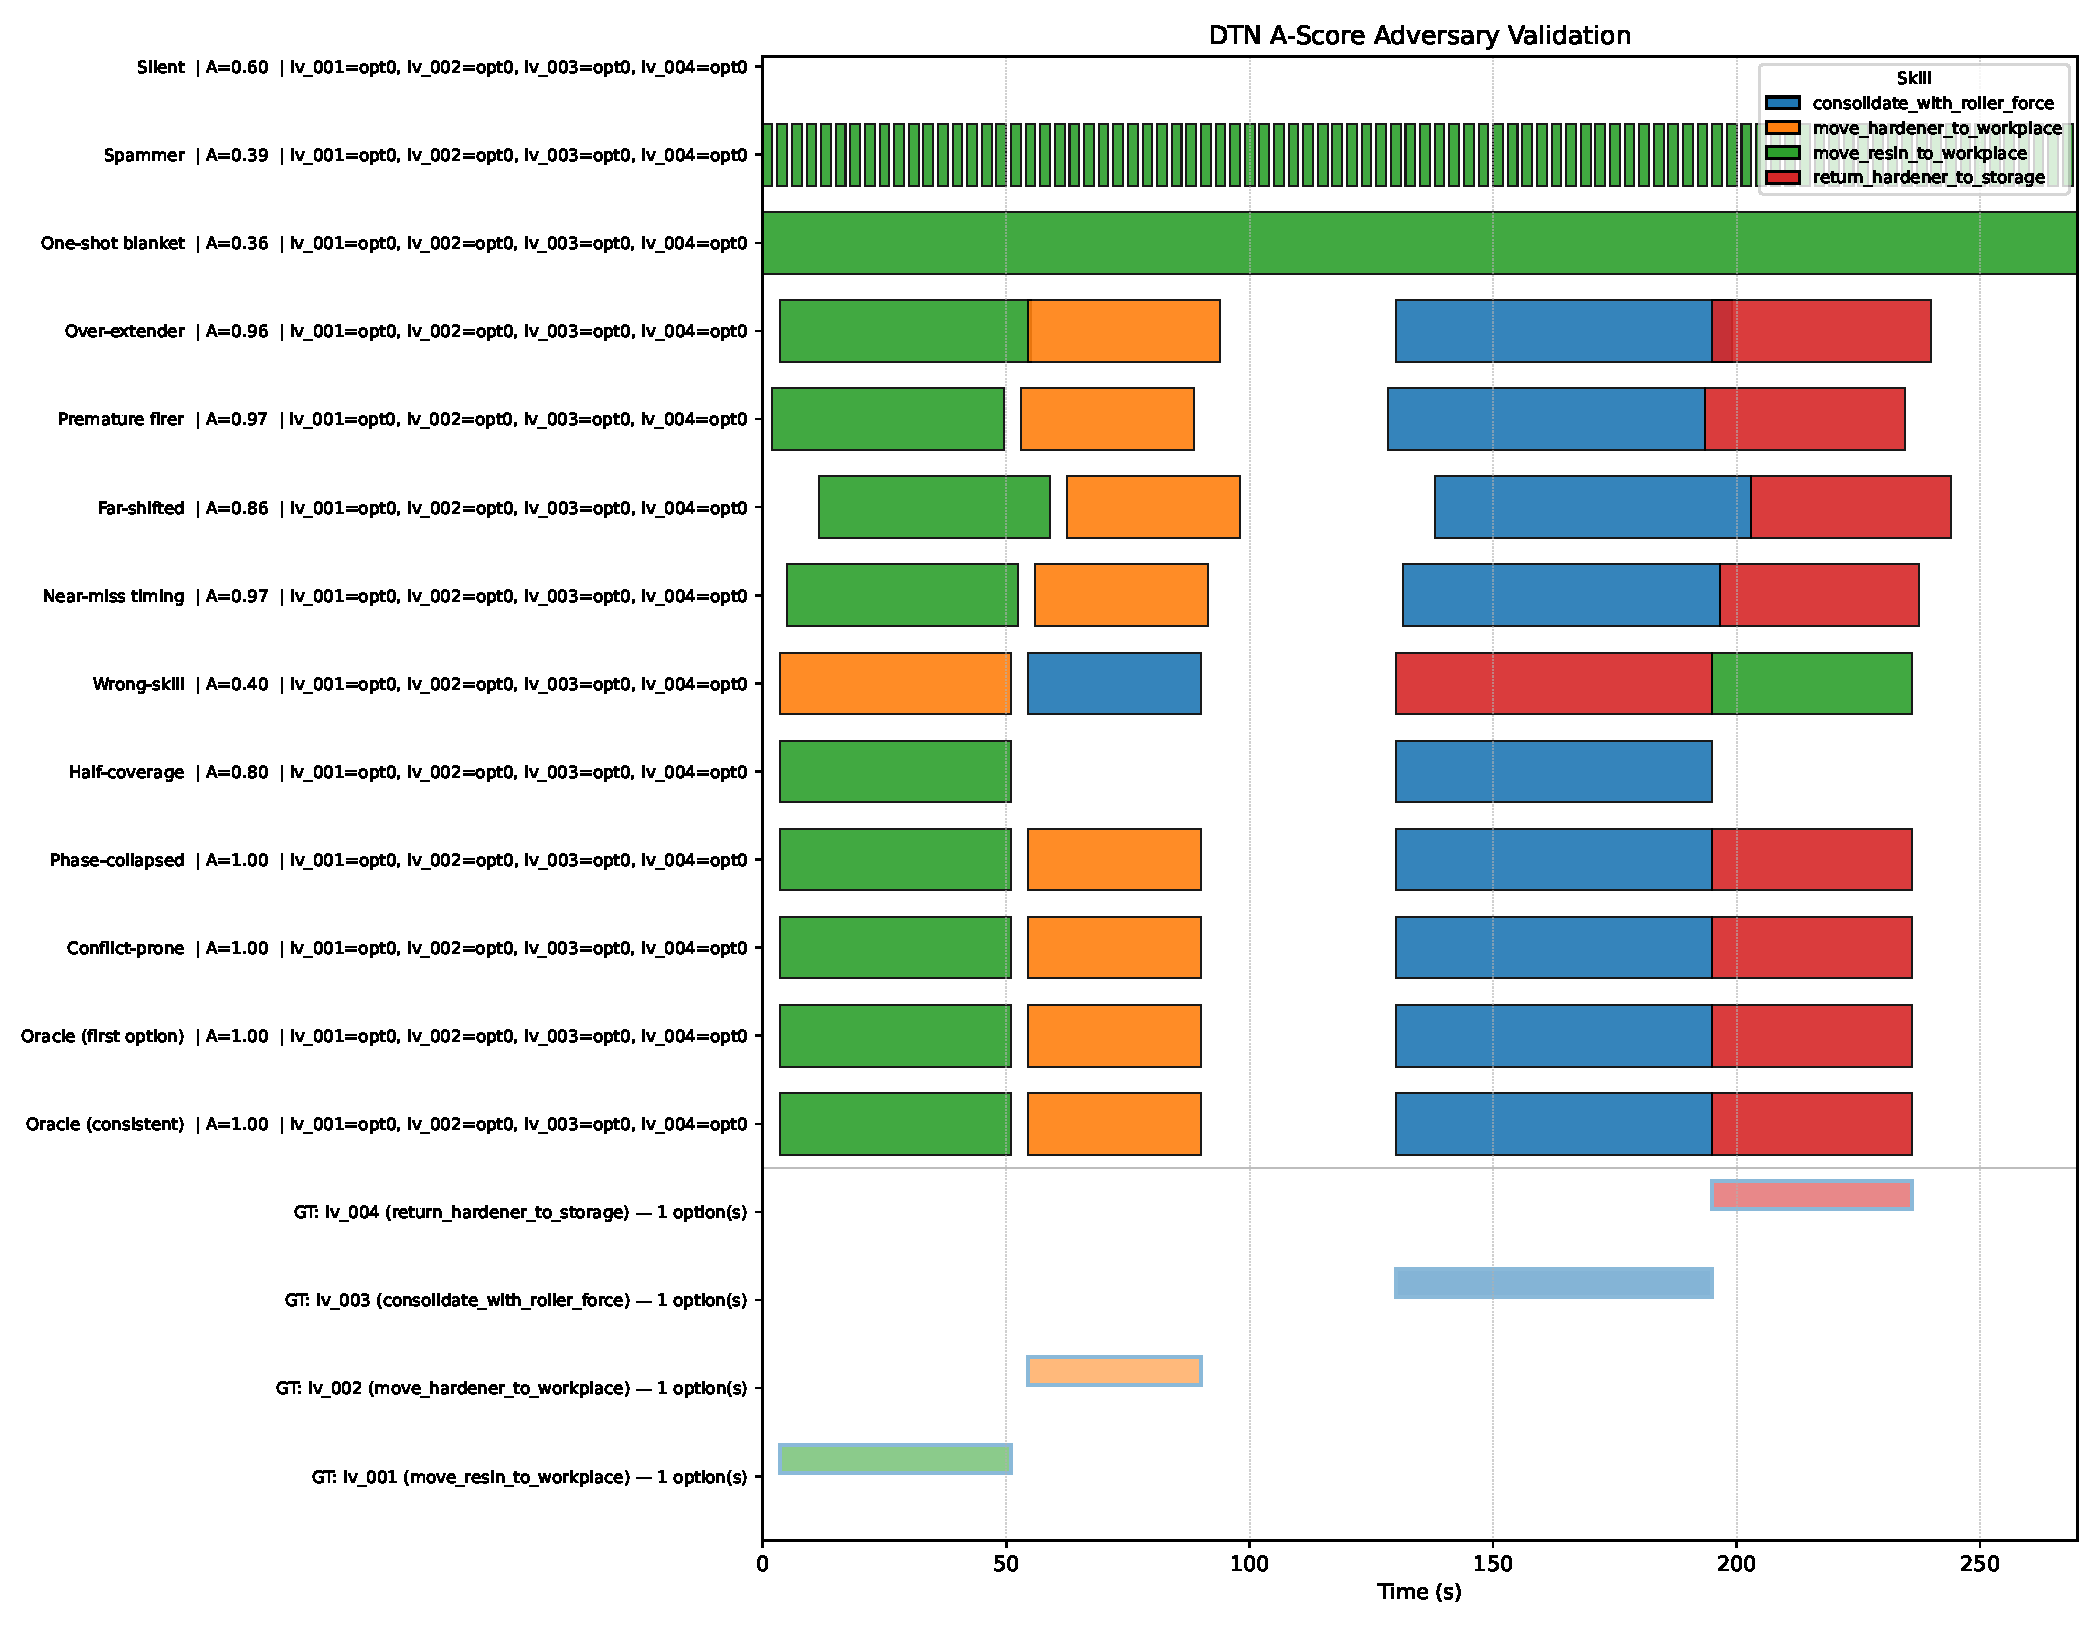
\includegraphics[width=\linewidth]{fig_dtn_adversaries_layup.pdf}
  \caption{Hand-layup ground truth (old format, one option / one
  phase per subtask). With nothing to choose between, $\Acons = 1$ for
  every adversary and the score reduces to a coverage-plus-action-plus-necessity
  blend.}
  \label{fig:layup}
\end{figure}

\begin{table}[ht]
\centering
\small
\begin{tabular}{lrrrrr}
\toprule
\textbf{Adversary} & $\bm{\Adisj}$ & $\bm{\Aact}$ & $\bm{\Acons}$ & $\bm{\Anec}$ & $\bm{\Score}$ \\
\midrule
Oracle (consistent)   & 1.00 & 1.00 & 1.00 & 1.00 & \textbf{1.00} \\
Oracle (first option) & 1.00 & 1.00 & 1.00 & 1.00 & 1.00 \\
Conflict-prone        & 1.00 & 1.00 & 1.00 & 1.00 & 1.00 \\
Phase-collapsed       & 1.00 & 1.00 & 1.00 & 1.00 & 1.00 \\
Half-coverage         & 0.50 & 1.00 & 1.00 & 1.00 & 0.80 \\
Wrong-skill           & 0.00 & 0.00 & 1.00 & 1.00 & 0.40 \\
Near-miss timing      & 0.94 & 1.00 & 1.00 & 0.98 & 0.97 \\
Far-shifted           & 0.70 & 1.00 & 1.00 & 0.90 & 0.86 \\
Premature firer       & 0.94 & 1.00 & 1.00 & 0.98 & 0.97 \\
Over-extender         & 0.92 & 1.00 & 1.00 & 0.94 & 0.96 \\
One-shot blanket      & 0.04 & 0.00 & 1.00 & 0.70 & 0.36 \\
Spammer               & 0.01 & 0.25 & 1.00 & 0.70 & 0.39 \\
Silent                & 0.00 & 1.00 & 1.00 & 1.00 & 0.60 \\
\bottomrule
\end{tabular}
\caption{Score breakdown on the hand-layup ground truth (old format,
one option / one phase per subtask).}
\label{tab:layup}
\end{table}

\section{Discussion}

\subsection{Why $\Acons$ is not just yes/no}
We could imagine a much harsher version of $\Acons$: 1 if the chosen
options fit together perfectly, 0 if there is any clash at all. We
chose a smoother version (1 minus the worst pair-IoU) because a
strategy that overlaps two phases by 1\% is qualitatively different
from one that fully collides on a 5-second window. The smooth version
still gives 1.0 for a feasible plan and 0.0 for a fully-conflicting
one --- but a near-miss is mostly fine.

\subsection{Why the silent strategy looks weird on the toy DTN}
On the toy DTN, the silent adversary scores $\Acons = 0$ rather than
the intuitive 1. This happens because, with no predictions to look
at, the option-selection logic falls back to ``option 0 for
everything'', and on the toy GT those options happen to clash. The
silent adversary is still ranked very low overall ($\Score = 0.4$)
because $\Adisj = 0$ dominates, so this is not a real bug --- but it
is a small wart that we could clean up by leaving $\Acons$ undefined
when no predictions match.

\subsection{Connection to the formal literature}
This work was inspired by Osanlou et al.~\cite{osanlou2022dtnu}, who
study \emph{Disjunctive Temporal Networks with Uncertainty} and ask
whether a strategy exists that can satisfy all constraints no matter
how the world unfolds. We are doing something simpler: we already
have a fixed prediction track and we just want to score it. We borrow
their constraint shape (equation~\ref{eq:dtn-constraint}) but not
their tree-search algorithm.

\section{Reproducibility}

The code lives in
\texttt{aura/scripts/eval/metric\_side\_quest/}:

\begin{itemize}
  \item \texttt{disjunctive\_gt.py} --- the new ground-truth dataclasses
    and a loader that also accepts old-format files.
  \item \texttt{dtn\_score.py} --- the four scoring axes plus a small
    backtracking solver used by the consistent-oracle adversary.
  \item \texttt{dtn\_adversaries.py} --- the thirteen adversaries and
    the command-line interface.
  \item \texttt{toy\_dtn\_three\_tasks.robot\_gt.json} --- the toy
    ground truth used in this note.
  \item \texttt{layup\_gesture\_demo\_stationary\_with\_overlay.robot\_gt.v2.json}
    --- new-format copy of the hand-layup ground truth (old-format
    file unchanged).
\end{itemize}

\noindent
To regenerate the figures and tables in this document:
\begin{lstlisting}
# Toy DTN (Figure 1, Table 2)
python scripts/eval/metric_side_quest/dtn_adversaries.py

# Hand-layup recording (Figure 2, Table 3)
python scripts/eval/metric_side_quest/dtn_adversaries.py \
    --gt scripts/eval/metric_side_quest/layup_gesture_demo_stationary_with_overlay.robot_gt.v2.json \
    --output scripts/eval/metric_side_quest/out/fig_dtn_adversaries_layup.pdf
\end{lstlisting}

\section{Conclusion}

We extended our robot-helper score to handle subtasks that admit more
than one acceptable schedule. The key idea is to describe each
subtask as a small ``or'' over options, where each option is itself
an ``and'' over time windows. The resulting score has four dimensions
--- coverage, action correctness, schedule consistency, and
necessity --- and the new \emph{consistency} dimension is what
captures the failure mode of picking options that clash on a
single-resource agent. We checked the score against thirteen
synthetic adversaries on a toy three-subtask example and on our
existing hand-layup recording. It ranks them sensibly and reduces to
the old behaviour when the ground truth is in the old format. The
next step is to plug it into the existing evaluation pipeline.

\begin{thebibliography}{1}

\bibitem{osanlou2022dtnu}
K.~Osanlou, J.~Frank, A.~Bursuc, T.~Cazenave, E.~Jacopin, C.~Guettier,
and J.~Benton.
\newblock Solving Disjunctive Temporal Networks with Uncertainty under
Restricted Time-Based Controllability using Tree Search and Graph
Neural Networks.
\newblock In \emph{Proceedings of the AAAI Conference on Artificial
Intelligence}, 2022.

\end{thebibliography}

\end{document}
